% -*- TeX:de -*-
\NeedsTeXFormat{LaTeX2e}
\documentclass[12pt,a4paper]{article}
\usepackage[german]{babel} % german text
\usepackage[DIV12]{typearea} % size of printable area
\usepackage[T1]{fontenc} % font encoding
%\usepackage[latin1]{inputenc} % most likely on Windows
\usepackage[utf8]{inputenc} % probably on Linux
\usepackage{multicol}

% PLOTTING
\usepackage{pgfplots} 
\usepackage{pgfplotstable}
\usepackage{url}
\usepackage{graphicx} % to include images
\usepackage{tikz}
\usepackage{subfigure} % for creating subfigures
\usepackage{amsmath} % a bunch of symbols
\usepackage{amssymb} % even more symbols
\usepackage{booktabs} % pretty tables
\usepackage{makecell} % multi row table heading

% a floating environment for circuits
\usepackage{float}
\usepackage{caption}

%\newfloat{circuit}{tbph}{circuits}
%\floatname{circuit}{Schaltplan}

% a floating environment for diagrams
%\newfloat{diagram}{tbph}{diagrams}
%\floatname{diagram}{Diagramm}

\selectlanguage{german} % use german

\begin{document}








%%%% TO DO
%
% - - Shorty:
%
% - - Tabelle "Messwerte Linsenbrennweite"
%		bitte bei jedem neuen e eine trennlinie... bin zu deppert ^^

% - - Patrick
%




%%%%%%% DECKBLATT %%%%%%%
\thispagestyle{empty}
			\begin{center}
			\Large{Fakultät für Physik}\\
			\end{center}
\begin{verbatim}


\end{verbatim}
							%Eintrag des Wintersemesters
			\begin{center}
			\textbf{\LARGE WS 2013/14}
			\end{center}
\begin{verbatim}


\end{verbatim}
			\begin{center}
			\textbf{\LARGE{Physikalisches Praktikum\\ für das Bachelorstudium}}
			\end{center}
\begin{verbatim}




\end{verbatim}

			\begin{center}
			\textbf{\LARGE{PROTOKOLL}}
			\end{center}
			
\begin{verbatim}





\end{verbatim}

			\begin{flushleft}
			\textbf{\Large{Experiment (Nr., Titel):}}\\
							%Experiment Nr. und Titel statt den Punkten eintragen
			\LARGE{PW7 Brechung, Dispersion, Refraktometrie}	
			\end{flushleft}

\begin{verbatim}

\end{verbatim}	
							%Eintragen des Abgabedatums, oder des Erstelldatums des Protokolls
			\begin{flushleft}
			\textbf{\Large{Datum:}} \Large{21.11.2013}
			\end{flushleft}
			
\begin{verbatim}
\end{verbatim}
							%Namen der Protokollschreiber
		\begin{flushleft}
			\textbf{\Large{Namen:}} \Large{Patrick Braun, Johannes Kurz}
			\end{flushleft}

\begin{verbatim}


\end{verbatim}
							%Kurstag und Gruppennummer, zb. Fr/5
			\begin{flushleft}
			\textbf{\Large{Kurstag/Gruppe:}} \Large{DO/2}
			\end{flushleft}

\begin{verbatim}



\end{verbatim}
							%Name des Betreuers, das Praktikum betreute.
			\begin{flushleft}
			\LARGE{\textbf{Betreuer:}}	\Large{ Johanna Akbarzadeh }	
			\end{flushleft}

%%%%%%% DECKBLATT ENDE %%%%%%%
\pagebreak
\setlength{\columnsep}{20pt}
\begin{multicols}{2}


%\begin{figure}[H]
%	\centering
%	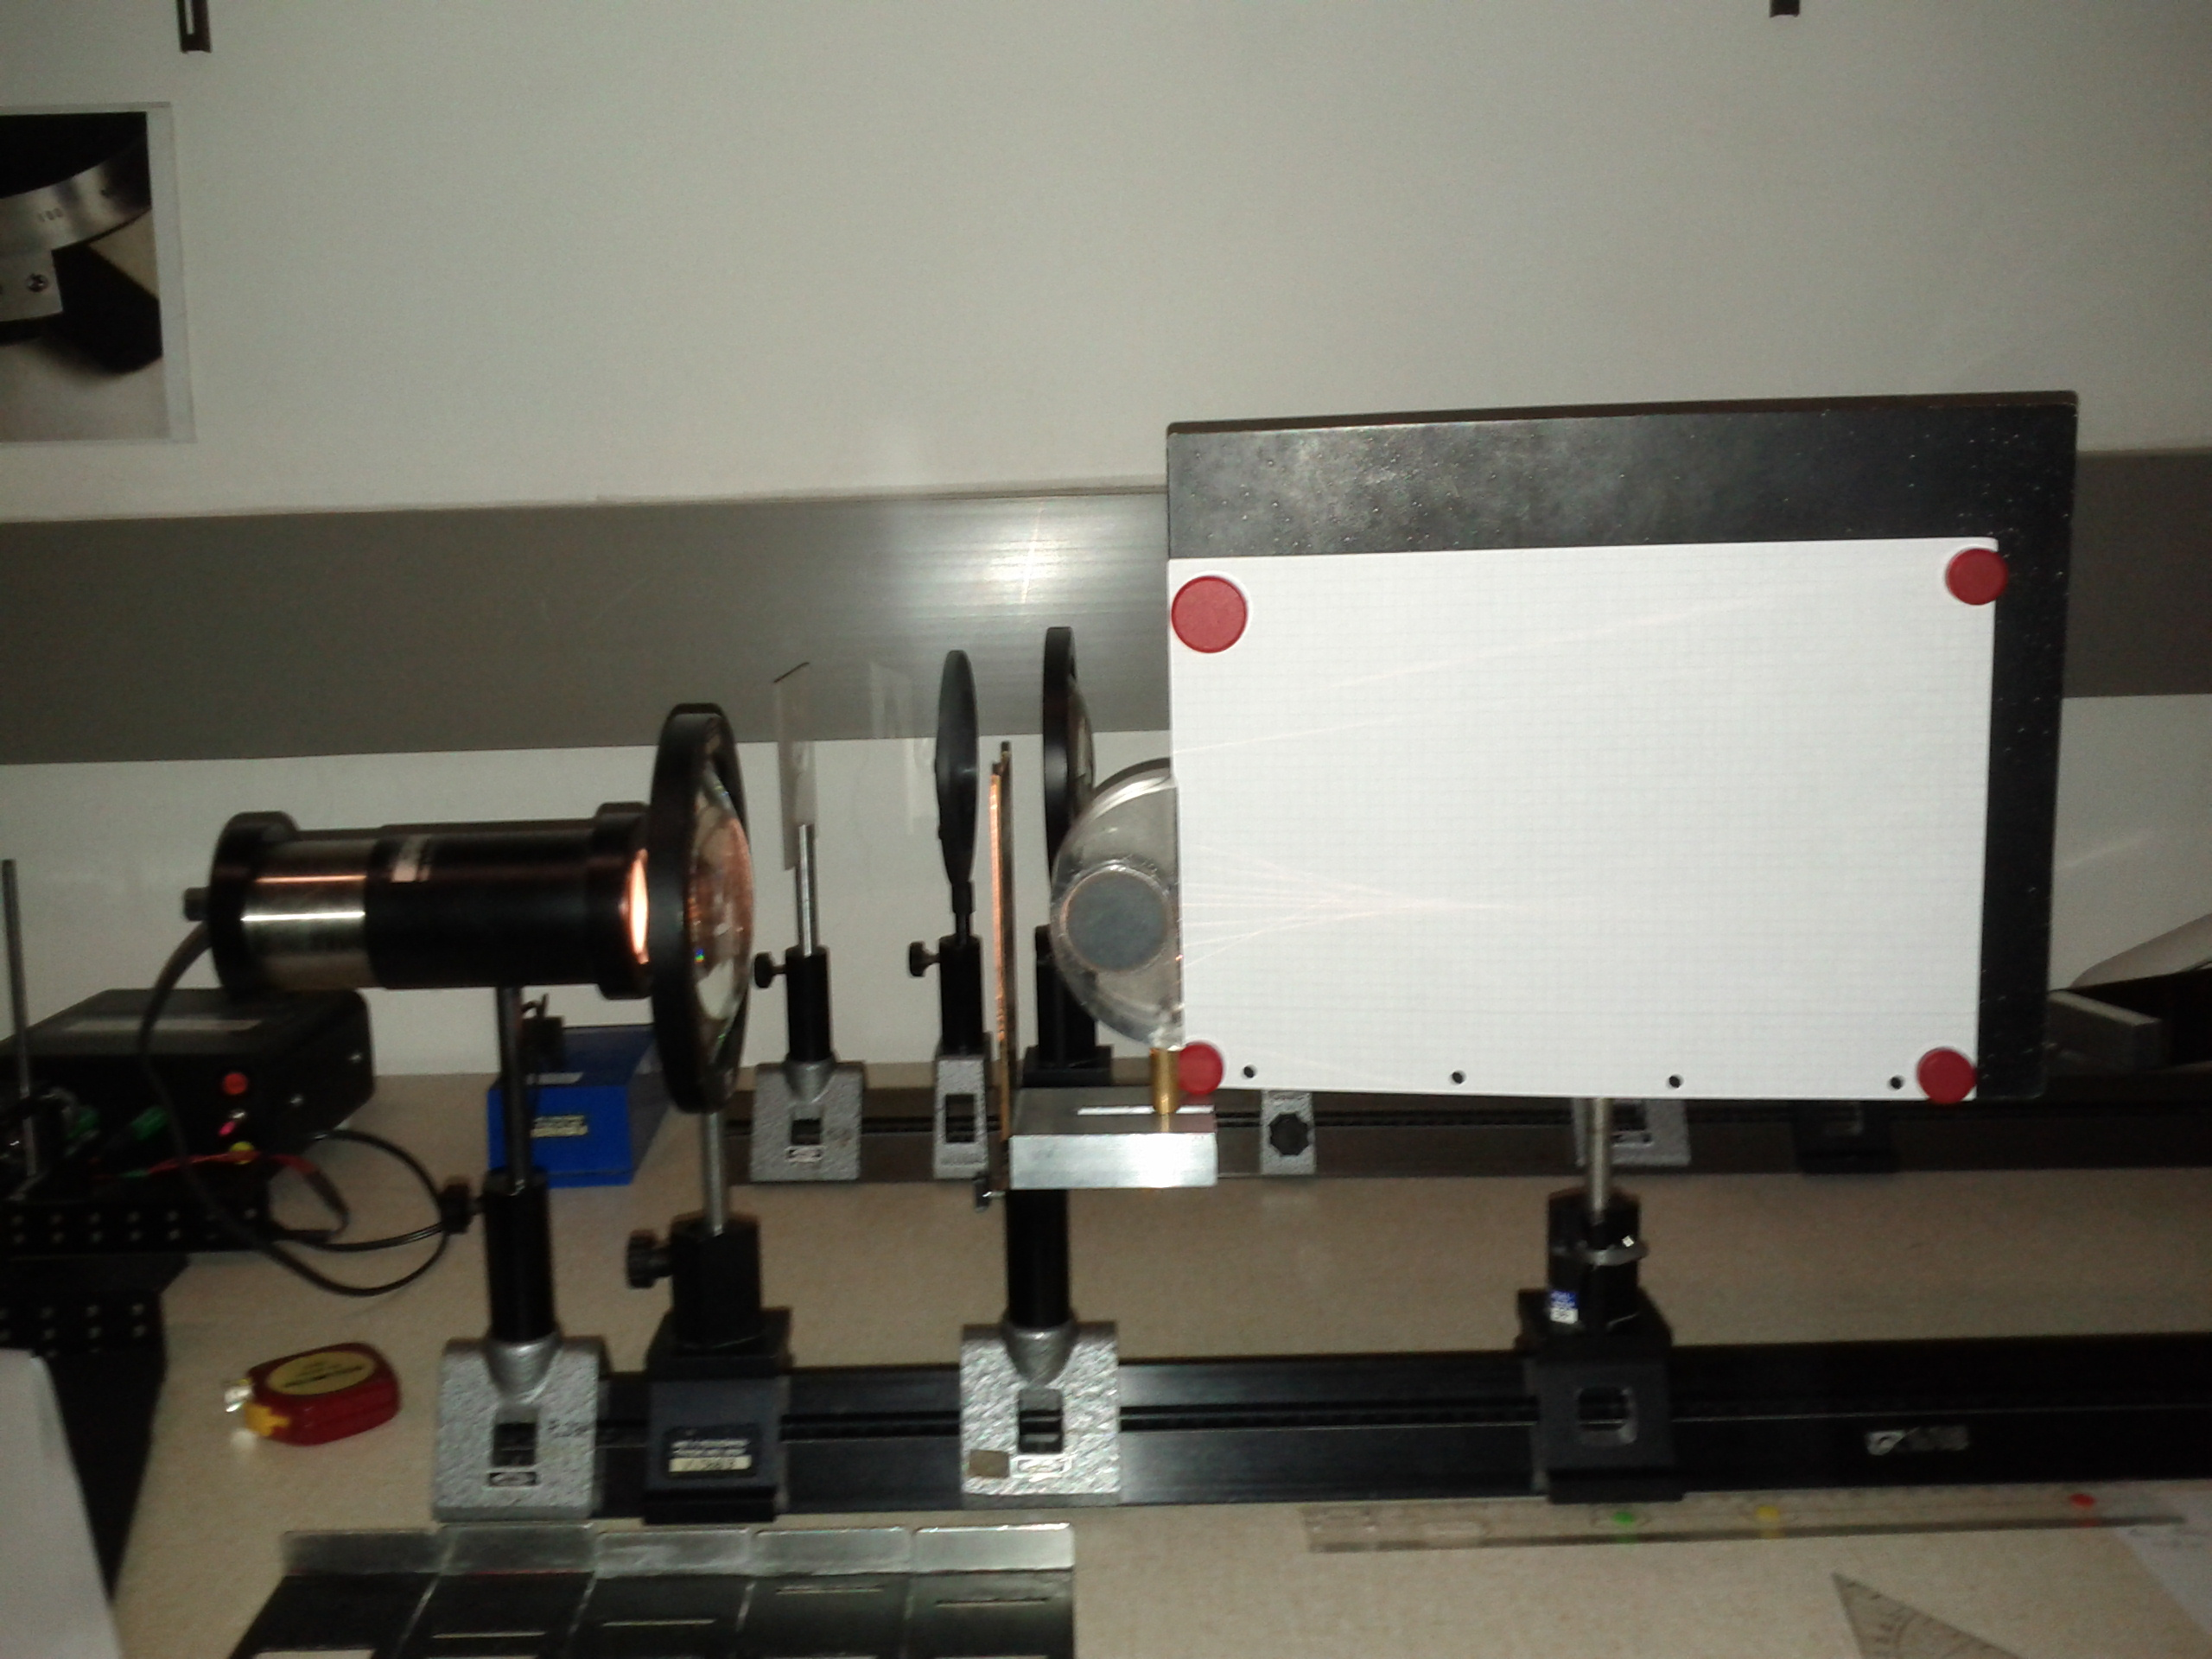
\includegraphics[scale=0.13]{./figure/linsenfehler.jpg}
%	\caption{Versuchaufbau Konvex-Plan Linse}
%	\label{fig:linsenfehler_aufbau}
%\end{figure}
%
%Glasprisma gegen Luft
%1.000292/sin(39grad28minutes)

%%%%%%%%%%%%%%%%%%%%%%%%%%%%%%%%%%%%%%%%%%%%%%%%
\section{Dispersionskurve eines Glasprismas}
%Cadmiumlampe, 5 Linien, 
Im ersten Experiment soll ein Glasprisma untersucht und seine Dispersionskurve gezeichnet werden.\\
Dabei wird eine Cadmium-Dampflampe verwendet, die ein diskretes Emissionsspektrum (mit 5 verschiedenen Wellenlängen) hat.\\
Ein Lichtstrahl dieser Lampe wird durch einen regelbaren Schlitz erzeugt und auf das Prisma gerichtet. Auch ist ein Fernrohr am Aufbau angebracht, welch, verbunden mit einem Goniometer, rotierbar ist. 
Durch das Einstellen des Null-Grad-Punktes (Lichtstrahl ohne Prisma) und anschließendes Rotieren des Prisma-Tisches, bis zu dem Punkt, an dem sich die Bewegung der jeweiligen Spektrallinie, trotz weiterer Rotation des Tisches, umkehrt, kann $\delta_{min}$ für alle Spektren bestimmt werden. \\
Der Versuchsaufbau mit Lampe, Blende, Prisma auf rotierbarem Tisch und Fernrohr ist in Abbildung \ref{fig:prisma_aufbau} ersichtlich.\\
%Der Brechungsindex ergibt sich durch:
%$$n = \frac{\sin{(\frac{\delta_{min} + \epsilon}{2})}}{\sin{(\frac{\epsilon}{2}})}$$
Zur Messung der Wellenlänge wurde ein mit einem Glasfaserkabel verbundener Sensor verwendet, welcher sich auf einem höhenverstellbarem Tisch befindet (zu sehen im Hintergrund von Abb.\ref{fig:prisma_aufbau}). Um diese Messung durchzuführen, wurde das Fernrohr weggeschwenkt und durch das Glasfaserkabel ersetzt. Das Prisma ist dabei nicht mehr notwendig.
\\ 
Die Wellenlängen der einzelnen Spektrallinien werden gegen ihren jeweiligen Brechungsindex aufgetragen. Es wird eine Kurve durch die Punkte gelegt, die den Brechungsindex des Prismas, abhängig von der Wellenlänge, angibt:

$$n(\lambda) = A + \frac{B}{\lambda^2}$$
\\


\begin{figure}[H]
	\centering
	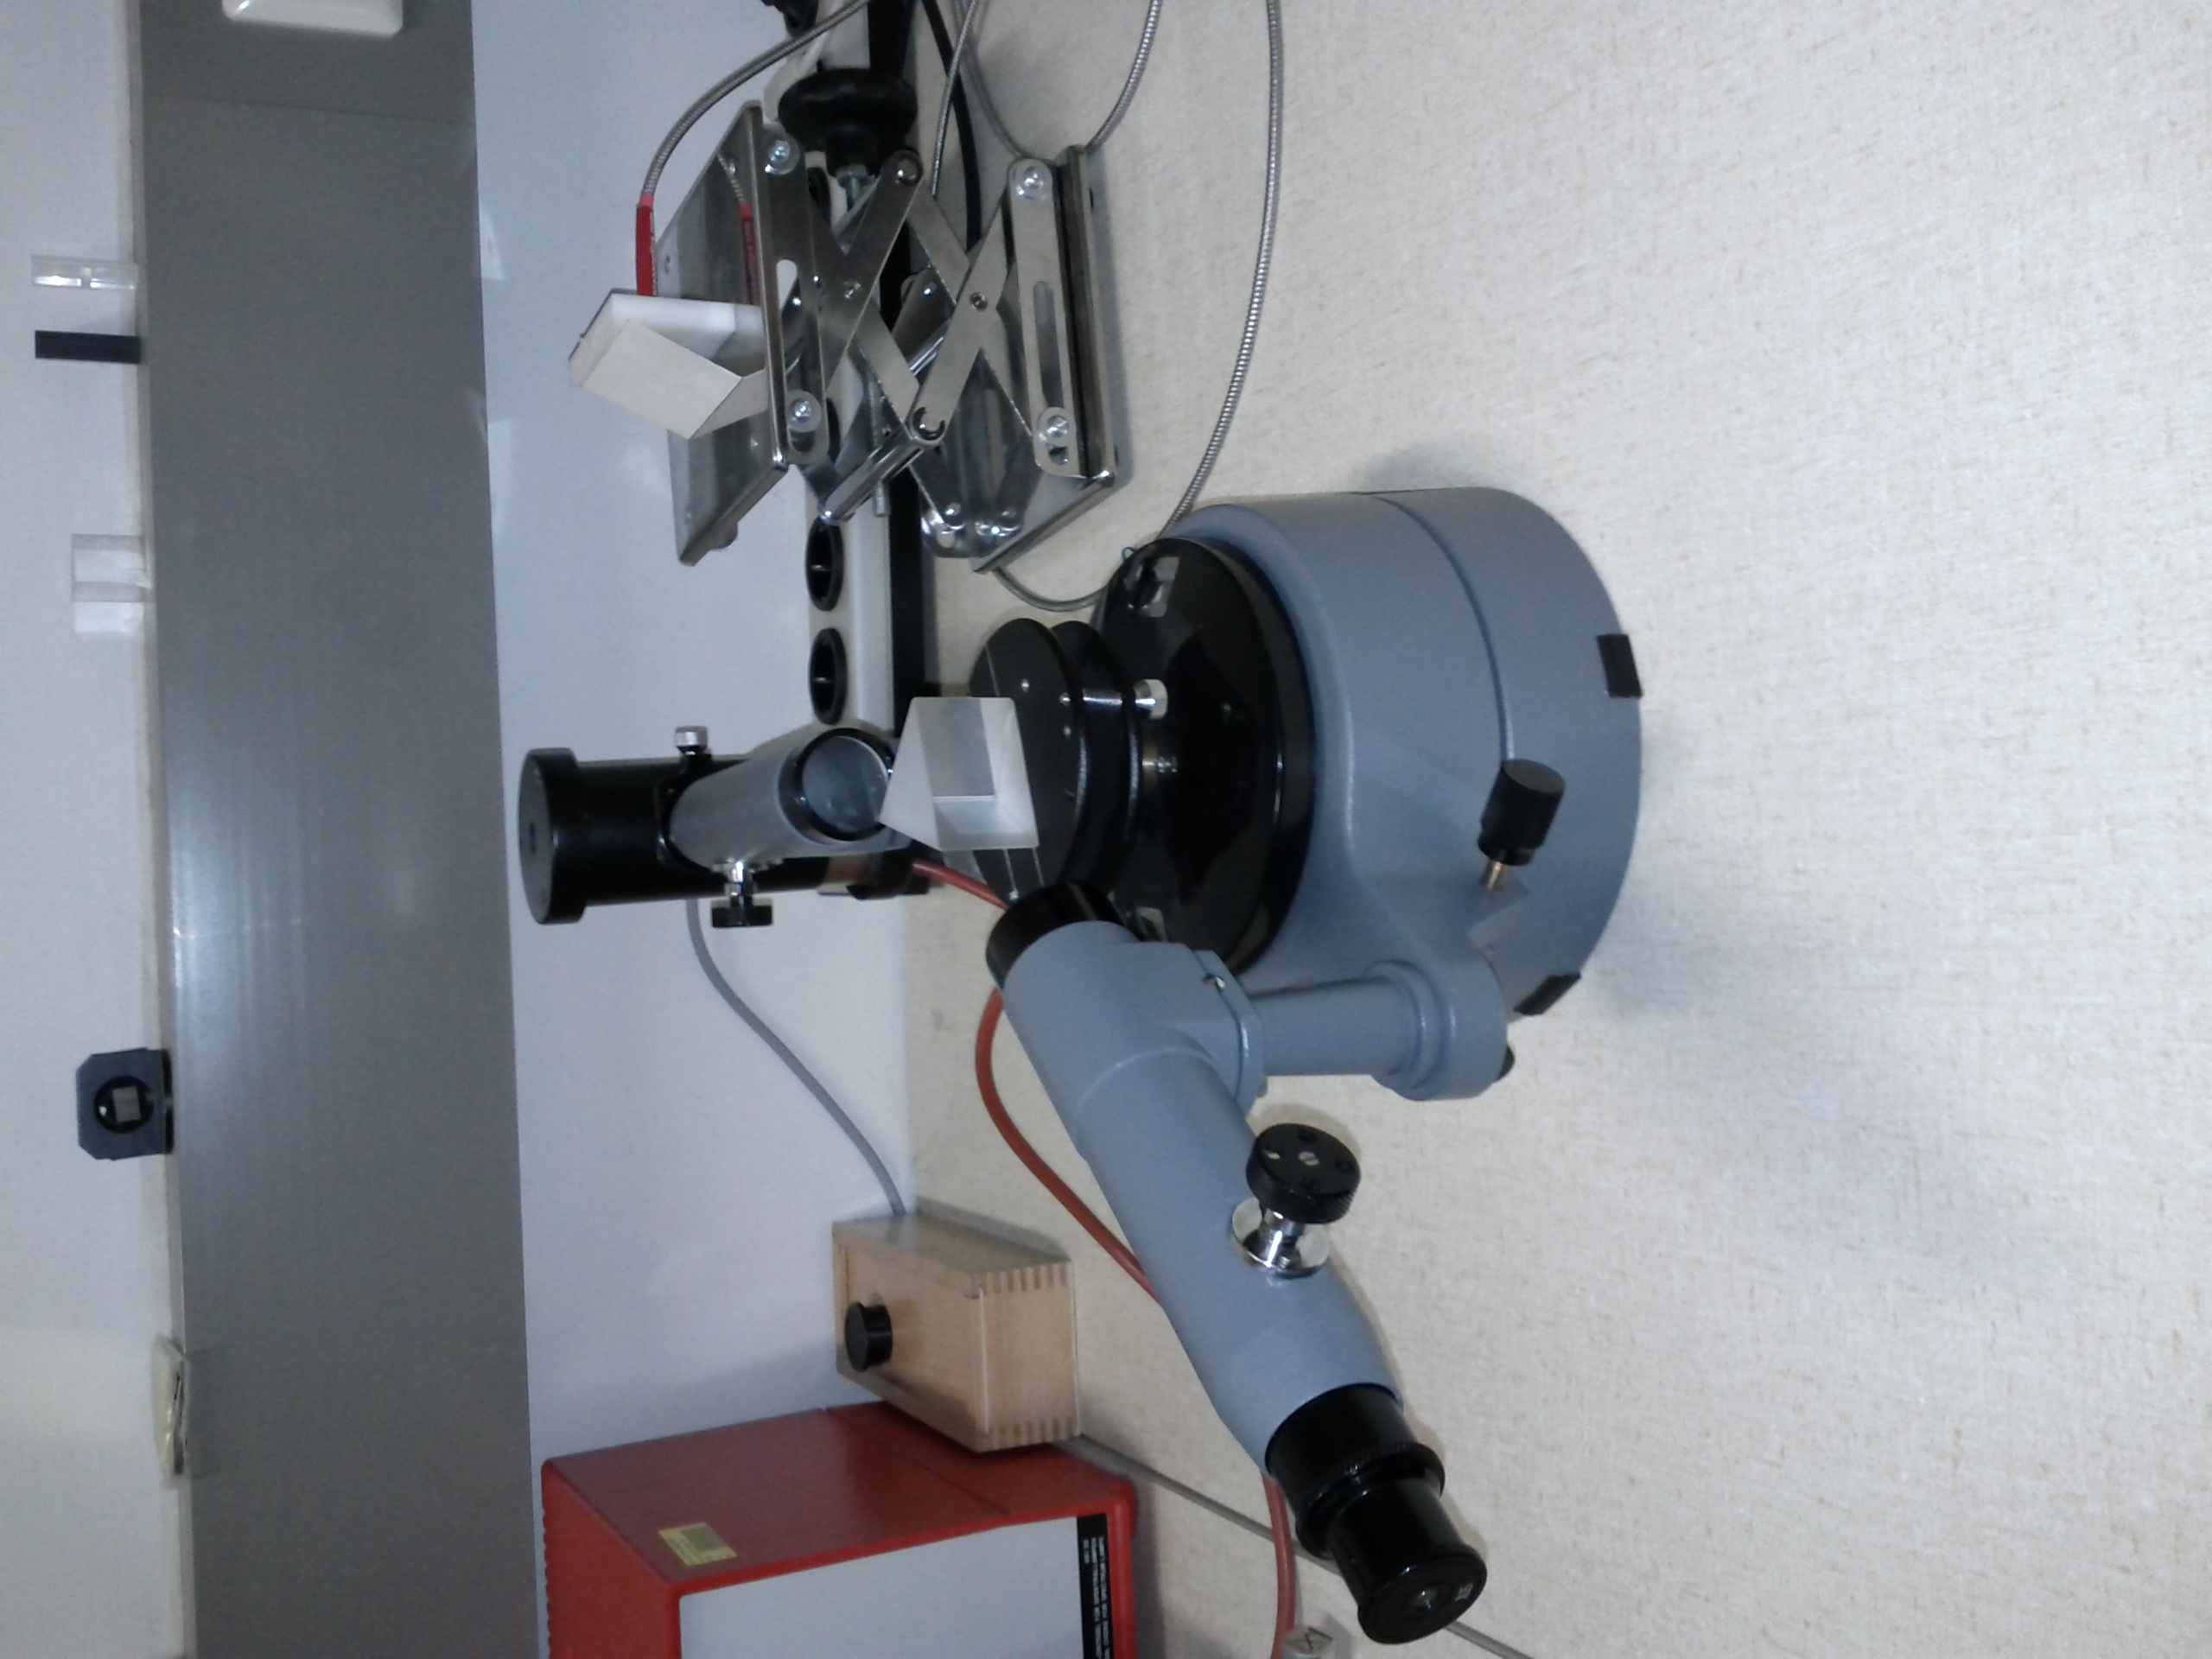
\includegraphics[angle=-90,scale=0.12]{./figure/prisma_aufbau.jpg}
	\caption{Versuchsaufbau Prisma}
	\label{fig:prisma_aufbau}
\end{figure}

\subsection{Messwerte und Ergebnisse}

\begin{figure}[H]
	\centering
	\pgfplotstabletypeset[
			columns={farbe, w,lambda},
			col sep=&,
			columns/farbe/.style={string type, column name=\makecell{$Farbe$\\} }, 
			columns/w/.style={string type, column name=\makecell{$Winkel$\\$[Grad]$} }, 
			columns/lambda/.style={column name=\makecell{$Wellenlänge$\\$[nm]$}, precision=0},
			every head row/.style={before row=\hline,after row=\hline\hline},
			every last row/.style={after row=\hline},
			every first column/.style={column type/.add={|}{} },
			every last column/.style={column type/.add={}{|} }
			]{
			farbe & w & lambda
			rot & 47$^\circ$ 39' & 543
			grün & 48$^\circ$ 58' & 508
			zyan & 49$^\circ$ 29' & 479
			blau & 49$^\circ$ 45' & 467
			violett & 50$^\circ$ 18' & 441
			
			}
	\caption{Farben, Winkel und Wellenlängen der Cadmium-Dampflampe}
	\label{fig:werte_cadmiumdampflampe}
\end{figure}
violett, 441nm: Literaturwert von der Betreuerin zur Verfügung gestellt, da der Peak im Sensor zu schwach war.

% TODO KURVE UND FORMEL ZUR RECHNUNG, Fehler

%A = 1,589733683934140e+00 +/- 9,033659153860940e-04
%B = 9,968439199611275e+03 +/- 2,159644777247912e+02

\end{multicols}
\begin{figure}[H]
	\centering
	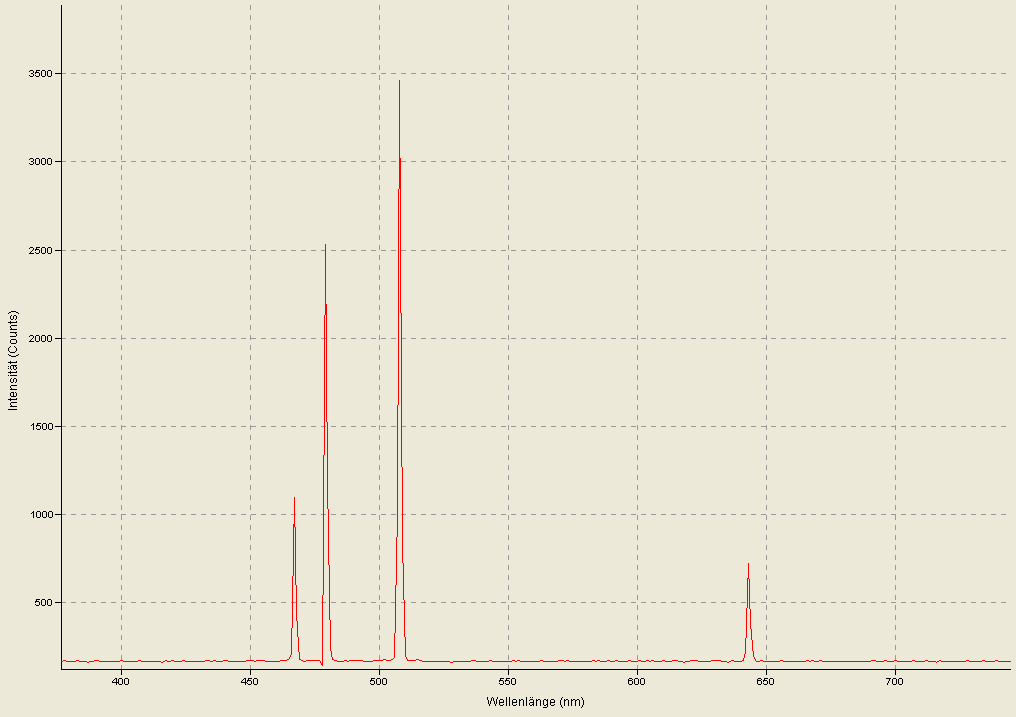
\includegraphics[scale=0.40]{./figure/Spektrum_Cadmiumdampflampe_PW7_Braun_Kurz.png}
	\caption{Spektrum Cadmiumlampe - Wellenlänge/Intensität}
	\label{fig:prisma_wellenlaenge}
\end{figure}

\begin{figure}[H]
	\centering
	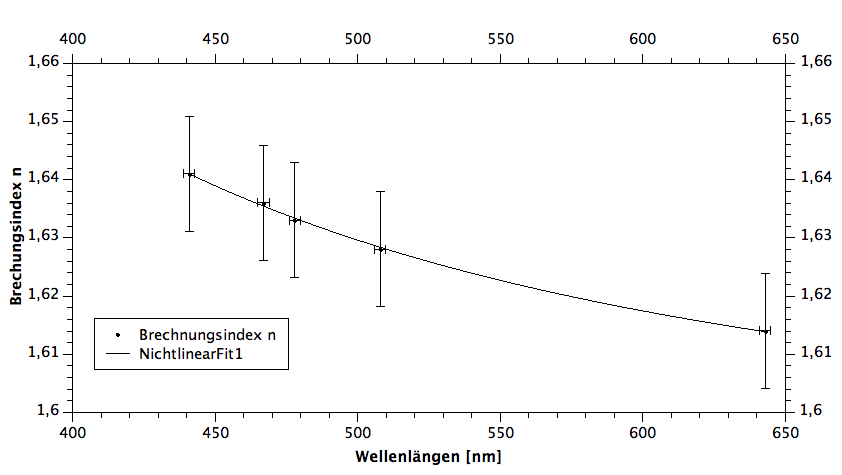
\includegraphics[scale=0.55]{./figure/anfpra7_spektrum_grafik.png}
	\caption{Brechungsindex abhängig von der Wellenlänge}
	\label{fig:wellenlaenge_brechungsindex}
\end{figure}

\begin{multicols}{2}

$$n(\lambda) = A + \sum_{j} \frac{B_j}{\lambda^{2j}}$$
%A = 1,589733683934140e+00 +/- 9,033659153860940e-04
%B = 9,968439199611275e+03 +/- 2,159644777247912e+02
$A=(1.58973 \pm 0.00091)$\\
$B_1 = (9970 \pm 220)nm^2$


\subsection{Diskussion}
%Dank neuem Equipment und leichter Bedienbarkeit war der Aufbau kein Problem. 
%Zu beachten ist eine genaue Nullpunktjustierung und die Mitte der Spektrallinien mit dem eingelassenen Fadenkreuz zu treffen um einen möglichst genauen Winkel messen zu können. 
%Dank dem Nonimus ist eine Minutengenaue Messung möglich. Durch die Justierungsmaßnahmen und das Treffen der Mitte einer Spektrallinie entsteht jedoch ein geschätzter Fehler von $\pm 5'$\\

Der Brechungsindex ergibt sich durch:
$$n = \frac{\sin{(\frac{\delta_{min} + \epsilon}{2})}}{\sin{(\frac{\epsilon}{2}})}$$
Der Nonius am Apparat erlaubt eine Messung auf Winkelminuten genau. Da jedoch die anvisierten Spektrallinien eine gewisse Breite haben und vor allem das Ablesen des Nonius, auch mit Lupe, etwas schwierig und sicher nicht exakt ist, wird die Unsicherheit am Winkel der minimalen Auslenkung mit $\pm 5'$ abgeschätzt.\\
Auf den Brechungsindex wirkt sich diese, mit etwa $\pm 0.050$, doch recht deutlich aus (siehe Fehlerbalken in Abb. \ref{fig:wellenlaenge_brechungsindex}).\\
Für eine Abschätzung von $\pm 2$ Winkelminuten würde sich die Unsicherheit des Brechungsindex auf $\pm 0.020$ reduzieren, und damit noch immer die gefittete Dispersionskurve deutlich beinhalten.\\
Dieser Genauigkeitsgewinn wäre zu erreichen durch bessere Lichtverhältnisse oder eine aufgehängte Lupe zur Ablesung, eine Digitalanzeige oder ähnliches. Abgesehen von Ableseschwierigkeiten sind die Autoren jedoch der Meinung, dass diese Genauigkeit mit diesem Aufbau problemlos erreichbar wäre.
\\
Die Messung der Wellenlängen durch den Sensor ist einfach aufzubauen und durchzuführen. Zu bemerken war, dass Umgebungslicht zu großen Störungen führt. Durch Abdunklung des Raumes konnten die Wellenlängen der Peaks mit vergleichsweise geringer Umgebungslichtverschmutzung gemessen werden (\ref{fig:prisma_wellenlaenge}).\\
Die Unsicherheit der Wellenlängen wurde abgeschätzt durch die halbe Breite des jeweiligen Peaks im Spektrum im unteren Drittel. Sie beträgt für die 4 gemessenen Spektrallinien jeweils $\pm 2nm$, und wurde auch für den violetten Messpunkt so übernommen.
\\
In Abbildung \ref{fig:wellenlaenge_brechungsindex} ist das Verhalten des Brechungsindex zur Wellenlänge aufgetragen. Die nichtlineare Funktion, mit der die Dispersionskurve angenähert wurde, liegt gut an den gemessenen Punkten. Weitere Glieder der Reihe sind also zur hinreichenden Beschreibung von $n(\lambda)$ ohne weitere Messpunkte (mit einer anderen Lampe) nicht nötig.

%%%%%%%%%%%%%%%%%%%%%%%%%%%%%%%%%%%%%%%%%%%%%%%%
\section{Lichtbrechung an einer planparallelen Platte}

Fällt Licht schräg durch eine Platte, wobei die Eintritts- und die Austritts-Grenzfläche parallel sind, wird ein Lichtstrahl 2 mal genau so gebrochen, dass er seine Richtung beibehält, aber um eine gewisse Distanz verschoben.\\
Der Strahl wird beim Eintritt zum Lot hin gebrochen, und beim Austritt im gleichen Verhältnis vom Lot weg, sodass der Strahl seinen ursprünglichen Winkel zur Platte beibehält (siehe Abb. \ref{fig:planparallele_Skizze}).\\
Dieser Umstand soll ausgenutzt werden, um mittels eines Mikroskops den Brechungsindex einer Glasplatte zu bestimmen: Sowohl an der Ober- als auch der Unterseite  der Platte sind Farbmarkierungen angebracht. Indem zuerst auf eine Markierung scharf gestellt wird, und danach auf eine der anderen Seite, lässt sich durch den Höhenunterschied des Objektivs die scheinbare Dicke der Platte feststellen, also diejenige $\delta$, die danke der Brechung des Lichtes wahrgenommen wird.\\
Der Höhenunterschied am Objektiv kann durch die Skalierung am Grobtrieb des Mikroskops abgelesen werden.\\
Außerdem wird die tatsächliche Dicke $d$ der Platte mit einer Mikrometerschraube an mehreren Stellen gemessen.\\
Das Verhältnis beider Längen entspricht dem Verhältnis der Tangens der beiden Brechungswinkel. Für kleine Winkel ist dieses auch gleich dem Verhältnis der beiden Sinus und damit dem Brechungsindex $n$ der Glasplatte.
$$\frac{\tan{\epsilon}}{\tan{\epsilon '}}=\frac{d}{b}\approx \frac{\sin{\epsilon}}{\sin{\epsilon '}}=n$$


\begin{figure}[H]
	\centering
	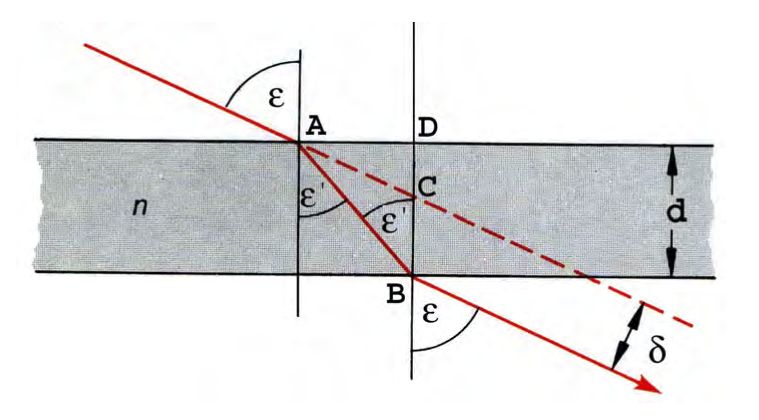
\includegraphics[scale=0.65]{./figure/planparallele_Skizze.png}
	\caption{Strahlengang in einer planparallelen Platte}
	\label{fig:planparallele_Skizze}
\end{figure}


\subsection{Messwerte und Ergebnisse}

\begin{figure}[H]
	\centering
	\pgfplotstabletypeset[
			columns={d,b},
			col sep=&,
			columns/d/.style={column name=\makecell{$d$\\$[mm]$}, precision=3, zerofill},
			columns/b/.style={column name=\makecell{$\delta$\\$[mm]$}, precision=3, zerofill},
			every head row/.style={before row=\hline,after row=\hline\hline},
			every last row/.style={after row=\hline},
			every first column/.style={
								column type/.add={|}{}
							        },
			every last column/.style={
								column type/.add={}{|}
								}
			]{
			b & d
			2.33 & 3.28
			2.205 & 3.29
			2.4 & 3.28
			2.355 & 3.26
			2.290 & 3.27
			
			}
	\caption{Messwerte für d (tatsächliche) und $\delta$ (scheinbare) Dicke}
	\label{fig:Messwerte_Glasplatte}
\end{figure}


\textbf{Ergebnis:}
\\
%$\delta = (2.316 \pm 0.033)mm$\\
$\delta = (2.3 \pm 0.1)mm$\\
$d = (3.28 \ pm 0.01)mm$

$$n = (1.426 \pm 0.063)$$



\subsection{Diskussion}

Bei der Messung der scheinbaren Dicke mit dem Mikroskop ist der Strahlengang fast senkrecht zur Platte, jedenfalls kleiner als 5$^\circ$. In dem Bereich ist die Kleinwinkel-Näherung sehr genau, außerdem sind die Fehler der Näherung für Sinus und Tangens in ihrer Richtung entgegengesetzt. Damit verringert sich der Fehler zusätzlich.\\
Die Unsicherheit für $\delta$ wurde mit 0.1mm bewusst groß gewählt. Während der Messung zeigte sich, dass bei 2-maligem Scharfstellen auf eine Markierung Unterschiede von  0.04mm zwischen den gewählten Positionen sind. Die subjektive Wahrnehmung von Schärfe verbunden mit einem ungeübten Blick dafür, bewirken also, dass diese Messung deutlich ungenauer ist, als es die Skalierung des Grobtriebes zulassen würde. \\
(Der standarderror of the mean für diese Messung wäre mit $\Delta \delta = 0.033mm$ kleiner, als die hier verwendeten 0.1mm und führen zu einer Unsicherheit $\Delta n = 0.021$, eben etwa 1/3 so groß.)\\
Die Messungen der tatsächlichen Dicke der Platte waren gleichmäßig verteilt und streuen nur schwach.\\
Die größte Quelle für Ungenauigkeiten ist in dieser Messung also sicherlich die menschliche Einschätzung, die vor allem durch Übung im Umgang mit dem Mikroskop zu verbessern wäre.\\
Das Ergebnis liegt jedenfalls im Bereich der Brechungsindizes für verschiedene Gläser [2], und dürfte damit valide sein.


%%%%%%%%%%%%%%%%%%%%%%%%%%%%%%%%%%%%%%%%%%%%%%%%
\section{Refraktometrie}
Ziel dieses Experiments ist es den Brechungsindex von Flüssigkeiten zu bestimmen. Zu diesem Zweck wird ein Abbe’sches Handrefraktometer (1) (Abb. \ref{fig:geraete_refrakto}, Vordergrund) und  ein Abbe’schen Refraktometer (2) (Abb.  \ref{fig:geraete_refrakto} Standgerät im Hintergrund) verwendet. 
\\
Im ersten Schritt wird der Brechungsindex des Messprismas im Handrefraktometer ohne Flüssigkeit bestimmt. Es wird der Winkel der Totalreflexion gemessen, der sich als hell/dunkel-Übergang erkennen und mit der angebrachten Winkelskala feststellen lässt. 
$$\sqrt{N^2-1}=\frac{\cos{\varphi}+\sin{i}}{\sin{\varphi}}$$
...wobei $\varphi = 61^\circ$ (aus der Anleitung PW7 [1] entnommen) und $i$ der Winkel der Totalreflexion ist.
\\
Zur Bestimmung des Brechungsindex der Messlinse wird monochromatischen Licht einer Na - Lampe verwendet.
\noindent
Danach wird die Probeflüssigkeit auf das Messprisma aufgebracht und das Beleuchtungsprisma aufgesetzt. Durch die Flüssigkeit ändert sich der Winkel der Totalreflexion, der nun wieder gemessen wird. 
\\
Dadurch ergibt sich aus den Gleichungen
\\
\\
\indent $n=N\cdot \sin{e}$\\
\indent $\sin i = N \cdot \sin r$\\
\indent $\varphi = r + e$
\\
\\
durch Umformung der Brechungsindex der Flüssigkeit. 
\\
Im Standgerät ist bereits eine geeichte Skala integriert, die ein direktes Ablesen des Brechungsindex ermöglicht.

\begin{figure}[H]
	\centering
	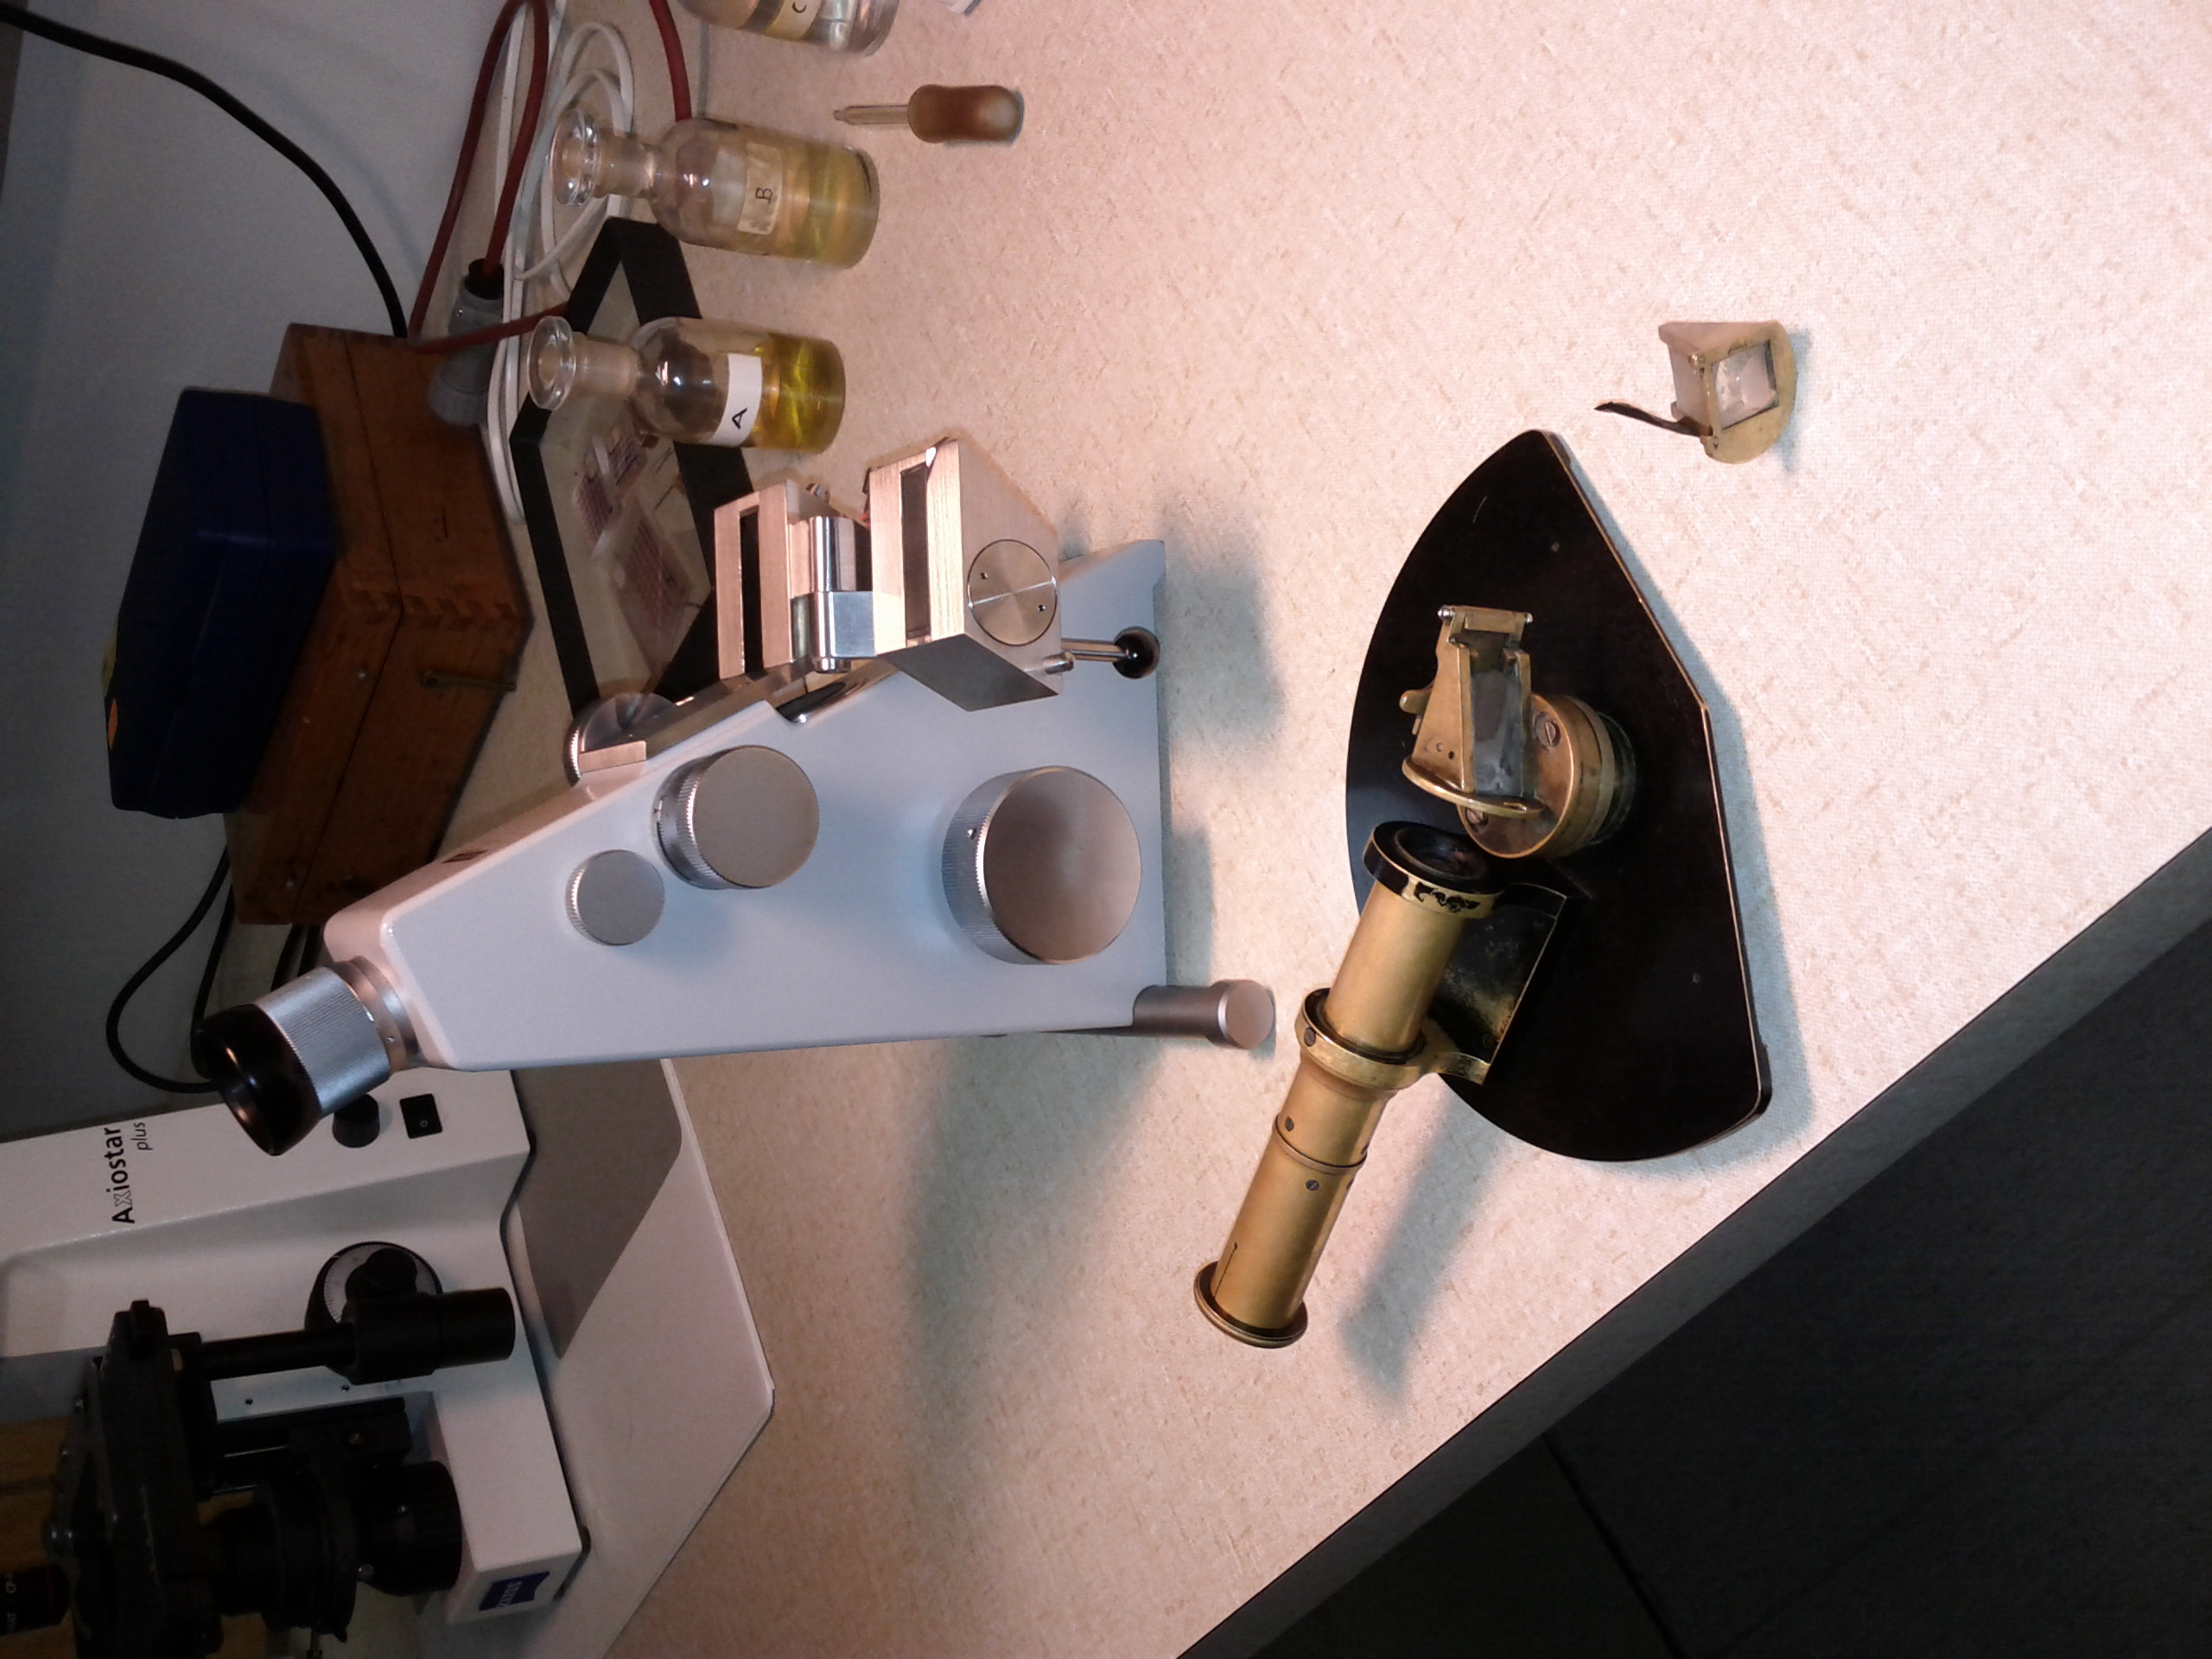
\includegraphics[angle=-90,scale=0.11]{./figure/refrakto.jpg}
	\caption{Verwendete Refraktometer}
	\label{fig:geraete_refrakto}
\end{figure}



\subsection{Messwerte und Ergebnisse}
Untersucht wurde die \textbf{Flüssigkeit B} mit dem Handrefraktometer (1): \\
\\
\textbf{Nulllage} des Refraktometers:\\
\indent $\phi_0 = 122^\circ 18'$\\
\textbf{Totalreflexion} des Messprismas:\\
\indent $\phi_{MT} = 161^\circ 46'$
%$$42' + 38^\circ + 46' = 39^\circ 28' = i$$
\indent $\Rightarrow i=39^\circ 28' $\\
%aus der Praktikums-Anleitung:\\
\indent $\phi_{Lot} = 61^\circ (Leitfaden)$\\
\\
\textbf{Brechungsindex} des Messprismas:
$$N_{Prisma} = 1.625$$%\footnote{Formel aus [1] (19)} $$
\\

\pagebreak

\noindent \textbf{Flüssigkeit B}:\\
$\phi_{FlüssigkeitB} = 128^\circ 20'$\\
\\
Nach Abziehen der Nulllage:\\
$i = 6^\circ 02'$\\
$e = 57^\circ 17'$\\
$r = 3^\circ 42'$
$$n_B = 1.367$$
\\
Nach der Brechungsindex-Tabelle (aus $[2]$), entspricht der ermittelte Brechungsindex am ehesten dem Literaturwert von Ethanol ($n_{Ethanol} = 1,3614$).\\
\\
\\
Messung von \textbf{Flüssigkeit B} mit dem \textbf{Standgerät (2)}:\\
$$n_B = (1.363 \pm 0.001)$$
\\
Außerdem wurde der Brechungsindex von \textbf{Flüssigkeit A} gemessen:\\
$$n_A = (1.358 \pm 0.001)$$
\\
% TODO Fehlerrechnung

\subsection{Diskussion}
Die Genauigkeit der Messung mit dem Handrefraktometer scheint durch alte Technik, ausgebrochener Prismen und Klebestreifen als Fixierung der Prismen beeinträchtigt. Tatsächlich ist ein Unterschied zur Messung mit dem moderneren Standgerät im Ergebnis für Flüssigkeit B erst ab der dritten Nachkommastelle festzustellen.\\

Die Unsicherheit des Ergebnisses aus der Zeiss-Standgerät-Messung wurde mit $\pm 0.001$ abgeschätzt. Das Gerät hätte eine Auflösung von $\pm 0.0005$, die auch gut erkennbar ist. Da jedoch vor allem mit dem älteren Handgerät verglichen werden soll, ist diese Genauigkeit in diesem Fall gar nicht erforderlich und lässt eine leicht vorsichtigere Abschätzung zu.
\\
\\
Die zusätzliche Messung der Flüssigkeit A hat beim ersten Versuch keine Totalreflexion hervorgerufen. Vermutlich rührt das aus einem Gemisch der Flüssigkeiten A und B in der Pipette her.\\
Nach Reinigung ergab sich in einer zweiten Messung der Wert wie angegeben. Dieser Brechungsindex entspricht in etwa dem von Aceton (aus [3]: $n_{Aceton}=1.359).$\\

An beiden Geräten ist die Grenze zwischen Brechung und Reflexion (hell/ dunkel) klar erkennbar. Da außerdem für die Flüssigkeit B beide Messungen übereinstimmen und die Ergebnisse nah an den Literaturwerten für Spiritus (B) bzw. Aceton (A) (Angaben durch die Betreuerin) liegen, gibt es wenig Grund, an den Ergebnissen zu zweifeln.


\section{Quellen}
$[1]$ Leitfaden, \url{http://www.univie.ac.at/anfpra/neu1/pw/pw7/PW7.pdf}\\
$[2]$ Brechungsindex \url{http://de.wikipedia.org/wiki/Brechungsindex}\\
$[3]$ Brechungsindex Aceton \url{http://www.chemicalbook.com/ChemicalProductProperty_DE_CB3130928.htm}

\end{multicols}
\end{document}